\documentclass{standalone}
\usepackage{tikz}

\begin{document}

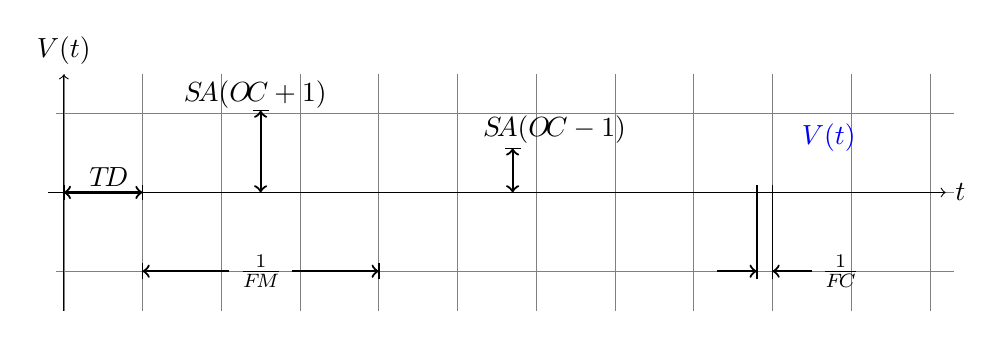
\begin{tikzpicture}[domain=0:11]
    %axes
    \draw[very thin,color=gray] (-0.1,-1.5) grid (11.3,1.5);
    \draw[->] (-0.2,0) -- (11.2,0) node[right] {$t$};
    \draw[->] (0,-1.5) -- (0,1.5) node[above] {$V(t)$};
    % MODULATOR in dashed red and formula
    \draw[dashed, color=red] plot[id=carrier1, samples=1000]
       function{.8*(1.3)*sin((x-1)*2*pi/3)*(x>=1 ? 1 : 0)} node[right] {};
    \draw[dashed, color=olive] plot[id=carrier2, samples=1000]
       function{.8*(.7)*sin((x-1)*2*pi/3)*(x>=1 ? 1 : 0)} node[right] {};
    %\draw[color=red] (3, 1.2)
    %   node[right] {$f(x) =\pm S\!A \sin \left[2\pi F\!M (t-T\!D)\right]$};
        %\draw[color=red] (3, 1.2)
       %node[right] {$f(x) =\pm V\!A \exp \left[-(t-T\!D)\cdot T\!H\!E\!T\!A\right] + V\!O$};
    % the time function
    \draw[color=blue, semithick] plot[id=am, samples=1000]
        function{.8*(.3+sin((x-1)*2*pi/3))*(sin((x-1)*2*pi*5))*(x>=1 ? 1 : 0)} 
        node[right] {};
    % the delay TD
    \draw[semithick, -] (0,-.1) -- (0,.1) node[] {};
    \draw[semithick, -] (1,-.1) -- (1,.1) node[] {};
    \draw[thick, <->] (0,0) -- (1,0) node[] {};
    \draw[] (.2,.2) node[right] {$T\!D$};
    % the amplitude SA(1+OC)
    \draw[semithick, -] (2.4,0) -- (2.6,0) node[] {};
    \draw[semithick, -] (2.4,1.04) -- (2.6,1.04) node[] {};
    \draw[thick, <->] (2.5,0) -- (2.5,1.04) node[] {};
    \draw[] (1.4,1.24) node[right] {$S\!A(O\!C+1)$};
    % the amplitude SA(-1+OC)
    \draw[semithick, -] (5.6,0) -- (5.8,0) node[] {};
    \draw[semithick, -] (5.6,.56) -- (5.8,.56) node[] {};
    \draw[thick, <->] (5.7,0) -- (5.7,.56) node[] {};
    \draw[] (5.2,.8) node[right] {$S\!A(O\!C-1)$};
    % no offset
    %\draw[] (0,.2) node[left] {$V\!O$};
    % FC
    \draw[thick, ->] (8.3,-1) -- (8.8,-1) node[] {};
    \draw[thick, <-] (9,-1) -- (9.5,-1) node[right] {$\frac{1}{F\!C}$};
    \draw[semithick, -] (8.8,-1.1) -- (8.8,0.1) node[] {};
    \draw[semithick, -] (9.,-1.1) -- (9.,0.1) node[] {};
    % FM
    \draw[semithick, -] (1,-1.1) -- (1,-.9) node[] {};
    \draw[semithick, -] (4,-1.1) -- (4,-.9) node[] {};
    \draw[thick, <-] (1,-1) -- (2.1,-1) node[right] {$\frac{1}{F\!M}$};
    \draw[thick, ->] (2.9,-1) -- (4,-1) node[] {};
    \draw[color=blue] (9.25,.7) node[right] {$V(t)$};
        %\draw[dashed, color=olive, semithick] (0,1.25) -- (5,0) node[] {};

\end{tikzpicture}

\end{document}
